Ved å ta en rekke forutsetninger om fremtidig utvikling, inntekter, kostnader og makroforhold har vi kommet frem til et resultat vi mener gjenspeiler nåverdien av investeringen. Likevel foreligger det stor usikkerhet rundt momentene fremvist i oppgaven. Det vil derfor presenteres ulike fremtidsbilder av investeringen med formål om å avdekke nåverdien gitt nye forutsetninger. Dette vil først belyses gjennom en \textit{best case} og \textit{worst case} analyse, før vi deretter undersøker hvor stor påvirkning de mest usikre momentene vil ha på nåverdien.

\section{Best case}
I denne delen velger vi utelukkende å endre veksten i salgsvolumet. Grunnen til at vi velger å bruke salgsvolum som endringsvariabel er at den påvirker både inntektene og kostnadene, og beskriver den fremtidige utviklingen best. I best case analysen anslår vi at salgsvolumet øker med 3\% de første 10 årene, deretter vil salgsvolumet avta og ligge stabilt på 1\% gjenværende tid. Dette gir en økning i nåverdien på 340,491 millioner. Internrenten med denne forutsetningen økes fra 28\% til 36\%.

\section{Worst case}
Worst case analysen legger også til grunn vekst i salgsvolum som endringsvariabel. For å beskrive en fremtidig utvikling som vi anser som verst, men fortsatt realistisk, bruker vi en årlig negativ vekst i salgsvolumet på 2\% de første 10 årene, før den synker til 3\% per år resterende tid. Basert på disse estimatene vil investeringen gi en negativ netto nåverdi på 18,758 millioner kroner.

\begin{table}[H]
  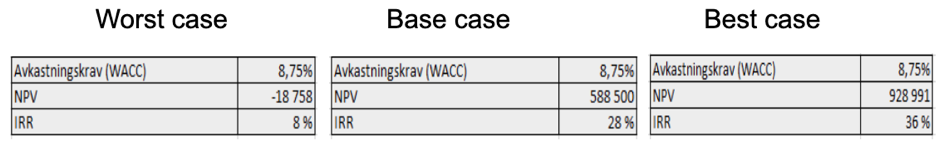
\includegraphics[width=\linewidth]{tabeller/case.png}
  \caption{Worst, Base og Best case oversikt}
  \label{tbl:case}
\end{table}

\section{Strømpris}
Strømprisen blir betraktet som en av de største merkostnadene til investeringen. Basert på historiske priser har denne vist seg å være ekstremt volatil, der man blant annet har opplevd en dobling i strømpris på kun ett år. Vår beregning tar utgangspunkt i en pris tilnærmet dagens nivå, med en økning på 0,25\% per år. Ved å endre denne prosentsatsen til 3\% vil netto nåverdien falle med omtrent 90 millioner. Investeringen vil fortsatt bli betraktet som svært lønnsom, og det er først ved en strømprisøkning på 10\% årlig at prosjektet gir en negativ avkastning.

\section{Totalkapitalkrav og levetid}
Avkastningskravet uttrykker usikkerheten i kontantstrømmene, og er derfor en av de mest utslagsgivende faktorene i vår analyse. Estimeringen av avkastningskravet har vært krevende å utforme, spesielt siden vi tillegger investeringen risiko utover selskapsrisikoen. Etter å ha utformet avkastningskravet basert på relevant teori kom vi frem til at investeringen hadde tilhørende risiko utover selskapets WACC. Vi behandlet dette ved å tillegge en prosentvis sats for henholdsvis business risk og valutarisiko. Ettersom disse satsene ble basert på skjønn er det nødvendig å foreta observasjoner av netto nåverdien der avkastningskravet settes både lavere og høyere enn det avkastningskravet vi har benyttet oss av.  

\begin{table}[H]
  \centering
  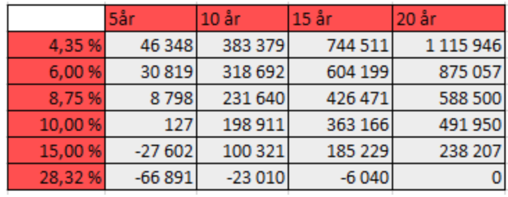
\includegraphics[scale=1.0]{tabeller/waccLevetid.png}
  \caption{WACC og levetid}
  \label{tbl:waccLevetid}
\end{table}

I tillegg til å legge inn nye avkastningskrav har vi også hensyntatt tidsperspektivet i denne analysen. I et fem-års perspektiv må avkastningskravet være 10\% for at investeringen ikke skal være lønnsom. Gjennom et 20-års perspektiv er investeringen lønnsom frem til og med internrenten som ligger på 28\%. Til tross for at lønnsomheten vil være positiv selv ved store endringer i avkastningskravet vil en endring på bare 1,25\% minske lønnsomheten med omtrent 100 millioner kroner. 

\section{Valutakurs}
Ettersom ROCKWOOL International er et multinasjonalt selskap, med hovedkontor i Danmark, vil kontantstrømmen kunne påvirkes av vekslingskursen mellom den norske og danske kronen. I modellen vår vil vi justere den estimerte nåverdien med diverse vekslingskurser. I tillegg til å bruke dagens kurs (Mai. 2019) har vi lagt ved ett utfall der den norske kronen svekkes mot den danske, ett der den norske kronen styrker seg mot den danske, og til slutt også gjennomsnittlig vekslingskurs de siste 5 årene, basert på månedlige observasjoner. I modellen legges det først til grunn at den danske kronekursen styrkes 10\% mot den norske, noe som fører til en ny netto nåverdi på 497,6 millioner danske kroner. Ved en dansk svekkelse med 10\% mot den norske kronen blir ny netto nåverdi 407,1 millioner danske kroner, noe som innebærer en differanse på omtrent 90 millioner danske kroner mot kronestyrkelsen. Dersom man legger til grunn en forventning om at den danske kronen vil ligne gjennomsnittet de siste fem årene vil netto nåverdien øke med omtrent 22 millioner for eierne. 


\begin{table}[H]
  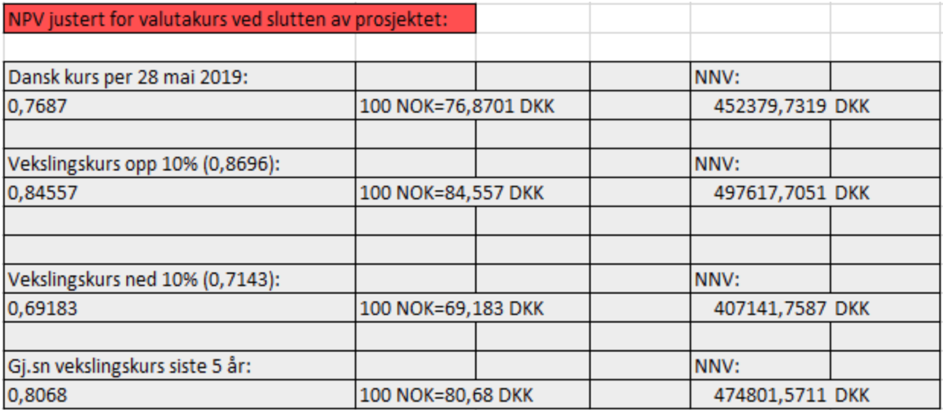
\includegraphics[width=\linewidth]{tabeller/NPVvaluta.png}
  \caption{NPV justert for valutakurs}
  \label{tbl:NPVvaluta}
\end{table}